\section{Рабочий проект}
\subsection{Спецификация системы}
\subsubsection{Модуль App.jsx}
Модуль App.jsx реализует главный компонент приложения, который управляет аутентификацией, начальной загрузкой данных и навигацией между различными представлениями приложения, такими как доска Kanban, профиль пользователя и страница аутентификации. Он координирует общее состояние приложения и обрабатывает глобальные задачи, такие как истечение сессии и обновление данных. В таблице \ref{appjsx:table} приведено описание состояний модуля.

\renewcommand{\arraystretch}{0.8}
\begin{xltabular}{\textwidth}{|X|X|}
	\caption{Описание состояний, используемых в App.jsx\label{appjsx:table}}\\
	\hline \centrow \setlength{\baselineskip}{0.7\baselineskip} Название состояния & \centrow \setlength{\baselineskip}{0.7\baselineskip} Описание состояния \\\hline
	\endfirsthead
	\caption*{Продолжение таблицы \ref{appjsx:table}}\\ \hline
	\finishhead
	isAuthenticated & Логический флаг для отслеживания, аутентифицирован ли пользователь в данный момент. \\ \hline
	isLoadingData & Логический флаг, указывающий, когда приложение находится в процессе загрузки начальных данных. \\ \hline
	isAddProjectModalOpenFromEmptyState & Логический флаг для управления видимостью модального окна Добавить проект, когда у пользователя нет проектов. \\ \hline
	tokenExpiredAlert & Состояние для модального окна оповещения об истечении срока действия токена, полученное из useStore. \\ \hline
	registrationAlert & Состояние для модального окна оповещения об успешной регистрации, полученное из useStore. \\ \hline
	projects & Массив, содержащий все проекты, доступные пользователю, полученный из useStore. \\ \hline
	currentProjectId & ID текущего выбранного проекта, полученный из useStore. \\ \hline
	dataRefreshTrigger & Счетчик, который при изменении запускает повторную загрузку данных, полученный из useStore. \\ \hline
	appView & Строка, определяющая текущее активное представление в приложении (например, kanban, profile), полученная из useStore. \\ \hline
	logoutConfirmModal & Состояние для модального окна подтверждения выхода, полученное из useStore. \\ \hline
\end{xltabular}

\subsubsection{Модуль index.css}
Модуль index.css реализует глобальные и утилитные стили для приложения с использованием Tailwind CSS. Он определяет базовые стили, пользовательские стили для полос прокрутки и корректировки макета для всего приложения.

\renewcommand{\arraystretch}{0.8}
\begin{xltabular}{\textwidth}{|X|X|}
	\caption{Описание параметров функций, используемых в index.css\label{indexcss:table}}\\
	\hline \centrow \setlength{\baselineskip}{0.7\baselineskip} Название параметра & \centrow \setlength{\baselineskip}{0.7\baselineskip} Описание параметра \\\hline
	\endfirsthead
	\caption*{Продолжение таблицы \ref{indexcss:table}}\\ \hline
	\finishhead
	\multicolumn{2}{|c|}{Нет} \\ \hline
\end{xltabular}

\subsubsection{Модуль main.jsx}
Модуль main.jsx реализует точку входа в приложение React. Он импортирует главный компонент App и глобальный CSS-файл, а затем отображает компонент App в элементе DOM с идентификатором root.

\subsubsection{Модуль store.js}
Модуль store.js реализует глобальное управление состоянием приложения с использованием Zustand. Он определяет центральное хранилище, включая переменные состояния и действия для управления проектами, досками, задачами, профилями пользователей, представлением приложения и различными состояниями пользовательского интерфейса, такими как модальные окна и оповещения. Он также включает в себя промежуточное ПО для сохранения частей состояния в локальное хранилище. В таблице \ref{storejs:table} приведено описание состояний модуля.

\renewcommand{\arraystretch}{0.8}
\begin{xltabular}{\textwidth}{|X|X|}
	\caption{Описание состояний, используемых в store.js\label{storejs:table}}\\
	\hline \centrow \setlength{\baselineskip}{0.7\baselineskip} Название состояния & \centrow \setlength{\baselineskip}{0.7\baselineskip} Описание состояния \\\hline
	\endfirsthead
	\caption*{Продолжение таблицы \ref{storejs:table}}\\ \hline
	\finishhead
	appView & Определяет текущее активное представление в приложении (например, kanban, profile, taskView). \\ \hline
	selectedTaskId & Хранит ID задачи, выбранной для детального просмотра. \\ \hline
	currentUserProfile & Хранит объект с данными профиля текущего вошедшего в систему пользователя. \\ \hline
	allUsers & Хранит список всех пользователей в системе, обычно для выпадающих списков назначения. \\ \hline
	mainLogoutHandler & Заполнитель для функции выхода из системы, который будет установлен компонентом App. \\ \hline
	dataRefreshTrigger & Счетчик, который можно увеличить для запуска повторной загрузки данных в компонентах. \\ \hline
	projects & Массив, содержащий все проекты, доступные пользователю. \\ \hline
	currentProjectId & ID текущего выбранного проекта. \\ \hline
	boards & Массив, содержащий все доски для всех проектов пользователя. \\ \hline
	tasks & Массив, содержащий все задачи для всех проектов пользователя. \\ \hline
	registrationAlert & Объект для управления состоянием модального окна оповещения о регистрации (показать, заголовок, сообщение). \\ \hline
	logoutConfirmModal & Объект для управления состоянием модального окна подтверждения выхода. \\ \hline
	tokenExpiredAlert & Объект для управления состоянием модального окна оповещения об истечении срока действия токена. \\ \hline
\end{xltabular}

\subsubsection{Модуль projectsPanel.jsx}
Модуль projectsPanel.jsx реализует компонент React, который отображает выпадающий список доступных проектов. Он позволяет пользователю просматривать и переключаться между различными проектами, обновляя текущий выбранный идентификатор проекта в приложении. В таблице \ref{projectspaneljsx:table} приведено описание состояний модуля.

\renewcommand{\arraystretch}{0.8}
\begin{xltabular}{\textwidth}{|X|X|}
	\caption{Описание состояний, используемых в projectsPanel.jsx\label{projectspaneljsx:table}}\\
	\hline \centrow \setlength{\baselineskip}{0.7\baselineskip} Название состояния & \centrow \setlength{\baselineskip}{0.7\baselineskip} Описание состояния \\\hline
	\endfirsthead
	\caption*{Продолжение таблицы \ref{projectspaneljsx:table}}\\ \hline
	\finishhead
	selectedProjectIdForDropdown & Хранит идентификатор проекта, выбранного в данный момент в выпадающем меню, для управления контролируемым вводом компонента. \\ \hline
\end{xltabular}

\subsubsection{Модуль settingsPanel.jsx}
Модуль settingsPanel.jsx реализует компонент боковой панели, который предоставляет действия пользователя и навигацию. Он включает кнопки для добавления задач, просмотра профиля пользователя, управления проектами и досками, а также выхода из системы. Доступ к определенным действиям контролируется на основе прав пользователя (владелец или администратор). В таблице \ref{settingspaneljsx:table} приведено описание состояний модуля.

\renewcommand{\arraystretch}{0.8}
\begin{xltabular}{\textwidth}{|X|X|}
	\caption{Описание состояний, используемых в settingsPanel.jsx\label{settingspaneljsx:table}}\\
	\hline \centrow \setlength{\baselineskip}{0.7\baselineskip} Название состояния & \centrow \setlength{\baselineskip}{0.7\baselineskip} Описание состояния \\\hline
	\endfirsthead
	\caption*{Продолжение таблицы \ref{settingspaneljsx:table}}\\ \hline
	\finishhead
	isAddBoardModalOpen & Логический флаг для управления видимостью модального окна Добавить доску. \\ \hline
	isAddProjectModalOpen & Логический флаг для управления видимостью модального окна Добавить проект. \\ \hline
	isEditProjectModalOpen & Логический флаг для управления видимостью модального окна Редактировать проект. \\ \hline
	isManageMembersModalOpen & Логический флаг для управления видимостью модального окна Управление участниками. \\ \hline
\end{xltabular}

\subsubsection{Модуль authPage.jsx}
Модуль authPage.jsx реализует компонент для аутентификации пользователя, обрабатывающий как вход, так и регистрацию. Он включает форму, которая динамически адаптируется для любого из этих представлений, с клиентской валидацией пользовательских вводов, таких как электронная почта и пароль. В таблице \ref{authpagejsx:table} приведено описание состояний модуля.

\renewcommand{\arraystretch}{0.8}
\begin{xltabular}{\textwidth}{|X|X|}
	\caption{Описание состояний, используемых в authPage.jsx\label{authpagejsx:table}}\\
	\hline \centrow \setlength{\baselineskip}{0.7\baselineskip} Название состояния & \centrow \setlength{\baselineskip}{0.7\baselineskip} Описание состояния \\\hline
	\endfirsthead
	\caption*{Продолжение таблицы \ref{authpagejsx:table}}\\ \hline
	\finishhead
	isRegisterView & Логический флаг для переключения между формами входа и регистрации. \\ \hline
	firstName & Хранит значение поля ввода имени для регистрации. \\ \hline
	lastName & Хранит значение поля ввода фамилии для регистрации. \\ \hline
	middleName & Хранит значение поля ввода отчества для регистрации. \\ \hline
	email & Хранит значение поля ввода электронной почты. \\ \hline
	password & Хранит значение поля ввода пароля. \\ \hline
	confirmPassword & Хранит значение поля подтверждения пароля для регистрации. \\ \hline
	showPassword & Логический флаг для переключения видимости пароля. \\ \hline
	isLoading & Логический флаг, указывающий, когда выполняется запрос на аутентификацию. \\ \hline
	firstNameError & Хранит сообщение об ошибке для поля имени. \\ \hline
	lastNameError & Хранит сообщение об ошибке для поля фамилии. \\ \hline
	emailError & Хранит сообщение об ошибке для поля электронной почты. \\ \hline
	passwordError & Хранит сообщение об ошибке для поля пароля. \\ \hline
	confirmPasswordError & Хранит сообщение об ошибке для поля подтверждения пароля. \\ \hline
	generalSubmitError & Хранит общее сообщение об ошибке при неудачной отправке формы. \\ \hline
	passwordCriteria & Массив объектов, представляющих критерии валидации пароля и их текущий статус (выполнено или нет). \\ \hline
	showPasswordCriteria & Логический флаг для управления видимостью списка требований к паролю. \\ \hline
\end{xltabular}

\subsubsection{Модуль taskPage.jsx}
Модуль taskPage.jsx реализует компонент, который отображает детальное представление одной выбранной задачи. Он показывает все атрибуты задачи, такие как описание, приоритет, срок выполнения и назначенных пользователей. Он также предоставляет действия для редактирования, удаления или назначения ролей для задачи. В таблице \ref{taskpagejsx:table} приведено описание состояний модуля.

\renewcommand{\arraystretch}{0.8}
\begin{xltabular}{\textwidth}{|X|X|}
	\caption{Описание состояний, используемых в taskPage.jsx\label{taskpagejsx:table}}\\
	\hline \centrow \setlength{\baselineskip}{0.7\baselineskip} Название состояния & \centrow \setlength{\baselineskip}{0.7\baselineskip} Описание состояния \\\hline
	\endfirsthead
	\caption*{Продолжение таблицы \ref{taskpagejsx:table}}\\ \hline
	\finishhead
	alertInfo & Объект для управления состоянием модального окна оповещения (показать, сообщение, заголовок). \\ \hline
	isEditModalOpen & Логический флаг для управления видимостью модального окна Редактировать задачу. \\ \hline
	isDeleteConfirmOpen & Логический флаг для управления видимостью модального окна подтверждения удаления. \\ \hline
\end{xltabular}

\subsubsection{Модуль userProfilePage.jsx}
Модуль userProfilePage.jsx реализует компонент, который отображает информацию о профиле текущего вошедшего в систему пользователя. Он извлекает данные пользователя и предоставляет опции для редактирования профиля или удаления учетной записи пользователя. В таблице \ref{userprofilepagejsx:table} приведено описание состояний модуля.

\renewcommand{\arraystretch}{0.8}
\begin{xltabular}{\textwidth}{|X|X|}
	\caption{Описание состояний, используемых в userProfilePage.jsx\label{userprofilepagejsx:table}}\\
	\hline \centrow \setlength{\baselineskip}{0.7\baselineskip} Название состояния & \centrow \setlength{\baselineskip}{0.7\baselineskip} Описание состояния \\\hline
	\endfirsthead
	\caption*{Продолжение таблицы \ref{userprofilepagejsx:table}}\\ \hline
	\finishhead
	isLoading & Логический флаг, указывающий, когда извлекаются данные профиля пользователя. \\ \hline
	error & Хранит любое сообщение об ошибке, возникающее при извлечении данных профиля. \\ \hline
	isEditModalOpen & Логический флаг для управления видимостью модального окна Редактировать профиль. \\ \hline
	isDeleteConfirmOpen & Логический флаг для управления видимостью модального окна подтверждения удаления учетной записи. \\ \hline
	generalAlert & Объект для управления состоянием общего модального окна оповещения (показать, сообщение, заголовок). \\ \hline
\end{xltabular}

\subsubsection{Модуль layoutObject.jsx}
Модуль layoutObject.jsx реализует основной компонент макета, который организует главный интерфейс приложения после входа в систему. Он объединяет панель настроек, панель проектов и основную область контента, которая может отображать либо представление доски Kanban, либо детальное представление задачи. Он также управляет логикой перетаскивания для задач и досок. В таблице \ref{layoutobjectjsx:table} приведено описание состояний модуля.

\renewcommand{\arraystretch}{0.8}
\begin{xltabular}{\textwidth}{|X|X|}
	\caption{Описание состояний, используемых в layoutObject.jsx\label{layoutobjectjsx:table}}\\
	\hline \centrow \setlength{\baselineskip}{0.7\baselineskip} Название состояния & \centrow \setlength{\baselineskip}{0.7\baselineskip} Описание состояния \\\hline
	\endfirsthead
	\caption*{Продолжение таблицы \ref{layoutobjectjsx:table}}\\ \hline
	\finishhead
	isAddTaskModalOpen & Логический флаг для управления видимостью модального окна Добавить задачу. \\ \hline
\end{xltabular}

\subsubsection{Модуль taskObject.jsx}
Модуль taskObject.jsx реализует одну карточку задачи на доске Kanban. Она перетаскиваемая и отображает ключевую информацию о задаче, такую как заголовок, тип, приоритет и срок выполнения. Нажатие на карточку переводит пользователя в детальное представление задачи. В таблицах \ref{taskobject1:table}, \ref{taskobject2:table} и \ref{taskobject3:table} приведено описание параметров функций модуля.

\renewcommand{\arraystretch}{0.8}
\begin{xltabular}{\textwidth}{|X|X|}
	\caption{Описание параметров функции TaskObject в taskObject.jsx\label{taskobject1:table}}\\
	\hline \centrow \setlength{\baselineskip}{0.7\baselineskip} Название параметра & \centrow \setlength{\baselineskip}{0.7\baselineskip} Описание параметра \\\hline
	\endfirsthead
	\caption*{Продолжение таблицы \ref{taskobject1:table}}\\ \hline
	\finishhead
	index & Индекс задачи в списке, используется для ключей и логики перетаскивания. \\ \hline
	state: taskProp & Объект, содержащий все данные для отображаемой задачи. \\ \hline
\end{xltabular}

\renewcommand{\arraystretch}{0.8}
\begin{xltabular}{\textwidth}{|X|X|}
	\caption{Описание параметров функции getCardBgColorByType в taskObject.jsx\label{taskobject2:table}}\\
	\hline \centrow \setlength{\baselineskip}{0.7\baselineskip} Название параметра & \centrow \setlength{\baselineskip}{0.7\baselineskip} Описание параметра \\\hline
	\endfirsthead
	\caption*{Продолжение таблицы \ref{taskobject2:table}}\\ \hline
	\finishhead
	typeValue & Строковое значение типа задачи (например, FRONTEND, BACKEND). \\ \hline
\end{xltabular}

\renewcommand{\arraystretch}{0.8}
\begin{xltabular}{\textwidth}{|X|X|}
	\caption{Описание параметров функции getUserShortDisplay в taskObject.jsx\label{taskobject3:table}}\\
	\hline \centrow \setlength{\baselineskip}{0.7\baselineskip} Название параметра & \centrow \setlength{\baselineskip}{0.7\baselineskip} Описание параметра \\\hline
	\endfirsthead
	\caption*{Продолжение таблицы \ref{taskobject3:table}}\\ \hline
	\finishhead
	userId & Числовой ID пользователя, информацию о котором нужно отобразить. \\ \hline
	rolePrefix & Строковый префикс для отображения перед именем пользователя (например, А:, Р:). \\ \hline
\end{xltabular}

\subsubsection{Модуль tooltipObject.jsx}
Модуль tooltipObject.jsx реализует многоразовый компонент, который предоставляет простую текстовую подсказку при наведении на любой дочерний элемент, который он оборачивает. В таблице \ref{tooltipobjectjsx:table} приведено описание состояний модуля.

\renewcommand{\arraystretch}{0.8}
\begin{xltabular}{\textwidth}{|X|X|}
	\caption{Описание состояний, используемых в tooltipObject.jsx\label{tooltipobjectjsx:table}}\\
	\hline \centrow \setlength{\baselineskip}{0.7\baselineskip} Название состояния & \centrow \setlength{\baselineskip}{0.7\baselineskip} Описание состояния \\\hline
	\endfirsthead
	\caption*{Продолжение таблицы \ref{tooltipobjectjsx:table}}\\ \hline
	\finishhead
	isVisible & Логический флаг для управления видимостью подсказки. \\ \hline
\end{xltabular}

\subsubsection{Модуль boardObject.jsx}
Модуль boardObject.jsx реализует одну колонку (доску) в представлении Kanban. Это перетаскиваемый контейнер, который содержит и отображает список задач. Он также предоставляет функциональность для редактирования деталей доски. В таблице \ref{boardobjectjsx:table} приведено описание состояний модуля.

\renewcommand{\arraystretch}{0.8}
\begin{xltabular}{\textwidth}{|X|X|}
	\caption{Описание состояний, используемых в boardObject.jsx\label{boardobjectjsx:table}}\\
	\hline \centrow \setlength{\baselineskip}{0.7\baselineskip} Название состояния & \centrow \setlength{\baselineskip}{0.7\baselineskip} Описание состояния \\\hline
	\endfirsthead
	\caption*{Продолжение таблицы \ref{boardobjectjsx:table}}\\ \hline
	\finishhead
	isModalEditOpen & Логический флаг для управления видимостью модального окна Редактировать доску для этой конкретной доски. \\ \hline
\end{xltabular}

\subsubsection{Модуль editBoardModal.jsx}
Модуль editBoardModal.jsx реализует модальный компонент для редактирования деталей (заголовка и описания) существующей доски. Он также содержит функциональность для удаления доски. В таблице \ref{editboardmodaljsx:table} приведено описание состояний модуля.

\renewcommand{\arraystretch}{0.8}
\begin{xltabular}{\textwidth}{|X|X|}
	\caption{Описание состояний, используемых в editBoardModal.jsx\label{editboardmodaljsx:table}}\\
	\hline \centrow \setlength{\baselineskip}{0.7\baselineskip} Название состояния & \centrow \setlength{\baselineskip}{0.7\baselineskip} Описание состояния \\\hline
	\endfirsthead
	\caption*{Продолжение таблицы \ref{editboardmodaljsx:table}}\\ \hline
	\finishhead
	title & Хранит значение поля ввода заголовка доски. \\ \hline
	description & Хранит значение поля ввода описания доски. \\ \hline
	isAlertOpen & Логический флаг для управления видимостью модального окна оповещения для уведомлений. \\ \hline
	alertMessage & Хранит сообщение, которое будет отображаться в модальном окне оповещения. \\ \hline
	populatedForBoardId & Хранит идентификатор доски, данные которой в настоящее время заполнены в модальном окне, чтобы предотвратить повторное отображение со старыми данными. \\ \hline
\end{xltabular}

\subsubsection{Модуль editProfileModal.jsx}
Модуль editProfileModal.jsx реализует модальный компонент, который позволяет текущему пользователю редактировать информацию своего профиля, такую как имя и URL-адрес аватара. В таблице \ref{editprofilemodaljsx:table} приведено описание состояний модуля.

\renewcommand{\arraystretch}{0.8}
\begin{xltabular}{\textwidth}{|X|X|}
	\caption{Описание состояний, используемых в editProfileModal.jsx\label{editprofilemodaljsx:table}}\\
	\hline \centrow \setlength{\baselineskip}{0.7\baselineskip} Название состояния & \centrow \setlength{\baselineskip}{0.7\baselineskip} Описание состояния \\\hline
	\endfirsthead
	\caption*{Продолжение таблицы \ref{editprofilemodaljsx:table}}\\ \hline
	\finishhead
	firstName & Хранит значение поля ввода имени. \\ \hline
	lastName & Хранит значение поля ввода фамилии. \\ \hline
	middleName & Хранит значение поля ввода отчества. \\ \hline
	avatarUrl & Хранит значение поля ввода URL-адреса аватара. \\ \hline
	isLoading & Логический флаг, указывающий, когда выполняется запрос на обновление профиля. \\ \hline
	errorAlert & Объект для управления состоянием модального окна оповещения об ошибке (показать, сообщение). \\ \hline
\end{xltabular}

\subsubsection{Модуль editProjectModal.jsx}
Модуль editProjectModal.jsx реализует модальный компонент для редактирования деталей (названия и описания) текущего выбранного проекта. Он также включает функциональность для удаления проекта. В таблице \ref{editprojectmodaljsx:table} приведено описание состояний модуля.

\renewcommand{\arraystretch}{0.8}
\begin{xltabular}{\textwidth}{|X|X|}
	\caption{Описание состояний, используемых в editProjectModal.jsx\label{editprojectmodaljsx:table}}\\
	\hline \centrow \setlength{\baselineskip}{0.7\baselineskip} Название состояния & \centrow \setlength{\baselineskip}{0.7\baselineskip} Описание состояния \\\hline
	\endfirsthead
	\caption*{Продолжение таблицы \ref{editprojectmodaljsx:table}}\\ \hline
	\finishhead
	projectName & Хранит значение поля ввода названия проекта. \\ \hline
	projectDescription & Хранит значение поля ввода описания проекта. \\ \hline
	isSubmitting & Логический флаг, указывающий, когда выполняется запрос на обновление или удаление. \\ \hline
	alertInfo & Объект для управления состоянием модального окна оповещения (показать, сообщение, заголовок). \\ \hline
	confirmDeleteModalOpen & Логический флаг для управления видимостью модального окна подтверждения удаления проекта. \\ \hline
	populatedForProjectId & Хранит идентификатор проекта, данные которого в настоящее время заполнены в модальном окне. \\ \hline
\end{xltabular}

\subsubsection{Модуль editTaskModal.jsx}
Модуль editTaskModal.jsx реализует модальный компонент для редактирования деталей существующей задачи, включая ее заголовок, описание, срок выполнения, статус (доску) и приоритет. В таблице \ref{edittaskmodaljsx:table} приведено описание состояний модуля.

\renewcommand{\arraystretch}{0.8}
\begin{xltabular}{\textwidth}{|X|X|}
	\caption{Описание состояний, используемых в editTaskModal.jsx\label{edittaskmodaljsx:table}}\\
	\hline \centrow \setlength{\baselineskip}{0.7\baselineskip} Название состояния & \centrow \setlength{\baselineskip}{0.7\baselineskip} Описание состояния \\\hline
	\endfirsthead
	\caption*{Продолжение таблицы \ref{edittaskmodaljsx:table}}\\ \hline
	\finishhead
	title & Хранит значение поля ввода заголовка задачи. \\ \hline
	description & Хранит значение поля ввода описания задачи. \\ \hline
	dueDate & Хранит значение поля ввода срока выполнения. \\ \hline
	selectedBoardId & Хранит идентификатор доски, выбранной для задачи. \\ \hline
	selectedPriority & Хранит уровень приоритета, выбранный для задачи. \\ \hline
	canEditDueDate & Логический флаг для определения, имеет ли текущий пользователь право редактировать срок выполнения. \\ \hline
	isAlertOpen & Логический флаг для управления видимостью модального окна оповещения. \\ \hline
	alertMessage & Хранит сообщение для модального окна оповещения. \\ \hline
	populatedForTaskId & Хранит идентификатор задачи, данные которой в настоящее время заполнены в модальном окне. \\ \hline
	minDate & Хранит минимально допустимую дату для выбора срока выполнения. \\ \hline
\end{xltabular}

\subsubsection{Модуль manageMembersModal.jsx}
Модуль manageMembersModal.jsx реализует модальный компонент для управления участниками проекта. Он позволяет владельцам проектов или администраторам просматривать, добавлять и удалять пользователей из текущего проекта. В таблице \ref{managemembersmodaljsx:table} приведено описание состояний модуля.

\renewcommand{\arraystretch}{0.8}
\begin{xltabular}{\textwidth}{|X|X|}
	\caption{Описание состояний, используемых в manageMembersModal.jsx\label{managemembersmodaljsx:table}}\\
	\hline \centrow \setlength{\baselineskip}{0.7\baselineskip} Название состояния & \centrow \setlength{\baselineskip}{0.7\baselineskip} Описание состояния \\\hline
	\endfirsthead
	\caption*{Продолжение таблицы \ref{managemembersmodaljsx:table}}\\ \hline
	\finishhead
	members & Массив для хранения списка текущих участников проекта. \\ \hline
	isLoadingMembers & Логический флаг, указывающий, когда извлекается список участников. \\ \hline
	emailToAdd & Хранит электронную почту пользователя для добавления в проект. \\ \hline
	isSubmitting & Логический флаг, указывающий, когда выполняется запрос на добавление или удаление участника. \\ \hline
	alertInfo & Объект для управления состоянием модального окна оповещения (показать, сообщение, заголовок). \\ \hline
\end{xltabular}

\subsubsection{Модуль modalObject.jsx}
Модуль modalObject.jsx реализует общий модальный компонент, используемый специально для создания новой задачи. Он предоставляет форму для ввода всех необходимых деталей задачи, таких как заголовок, описание, доска, приоритет и срок выполнения. В таблице \ref{modalobjectjsx:table} приведено описание состояний модуля.

\renewcommand{\arraystretch}{0.8}
\begin{xltabular}{\textwidth}{|X|X|}
	\caption{Описание состояний, используемых в modalObject.jsx\label{modalobjectjsx:table}}\\
	\hline \centrow \setlength{\baselineskip}{0.7\baselineskip} Название состояния & \centrow \setlength{\baselineskip}{0.7\baselineskip} Описание состояния \\\hline
	\endfirsthead
	\caption*{Продолжение таблицы \ref{modalobjectjsx:table}}\\ \hline
	\finishhead
	selectedBoardId & Хранит идентификатор доски, выбранной для новой задачи. \\ \hline
	selectedPriority & Хранит уровень приоритета, выбранный для новой задачи. \\ \hline
	selectedType & Хранит тип, выбранный для новой задачи. \\ \hline
	title & Хранит значение поля ввода заголовка новой задачи. \\ \hline
	description & Хранит значение поля ввода описания новой задачи. \\ \hline
	dueDate & Хранит значение поля ввода срока выполнения для новой задачи. \\ \hline
	minDate & Хранит минимально допустимую дату для выбора срока выполнения. \\ \hline
	isAlertOpen & Логический флаг для управления видимостью модального окна оповещения. \\ \hline
	alertMessage & Хранит сообщение для модального окна оповещения. \\ \hline
\end{xltabular}

\subsubsection{Модуль addBoardModal.jsx}
Модуль addBoardModal.jsx реализует модальный компонент, который предоставляет форму для создания новой доски (колонки) в текущем выбранном проекте. В таблице \ref{addboardmodaljsx:table} приведено описание состояний модуля.

\renewcommand{\arraystretch}{0.8}
\begin{xltabular}{\textwidth}{|X|X|}
	\caption{Описание состояний, используемых в addBoardModal.jsx\label{addboardmodaljsx:table}}\\
	\hline \centrow \setlength{\baselineskip}{0.7\baselineskip} Название состояния & \centrow \setlength{\baselineskip}{0.7\baselineskip} Описание состояния \\\hline
	\endfirsthead
	\caption*{Продолжение таблицы \ref{addboardmodaljsx:table}}\\ \hline
	\finishhead
	title & Хранит значение поля ввода заголовка новой доски. \\ \hline
	description & Хранит значение поля ввода описания новой доски. \\ \hline
	isAlertOpen & Логический флаг для управления видимостью модального окна оповещения. \\ \hline
	alertMessage & Хранит сообщение для модального окна оповещения. \\ \hline
\end{xltabular}

\subsubsection{Модуль addProjectModal.jsx}
Модуль addProjectModal.jsx реализует модальный компонент, который предоставляет форму для создания нового проекта. В таблице \ref{addprojectmodaljsx:table} приведено описание состояний модуля.

\renewcommand{\arraystretch}{0.8}
\begin{xltabular}{\textwidth}{|X|X|}
	\caption{Описание состояний, используемых в addProjectModal.jsx\label{addprojectmodaljsx:table}}\\
	\hline \centrow \setlength{\baselineskip}{0.7\baselineskip} Название состояния & \centrow \setlength{\baselineskip}{0.7\baselineskip} Описание состояния \\\hline
	\endfirsthead
	\caption*{Продолжение таблицы \ref{addprojectmodaljsx:table}}\\ \hline
	\finishhead
	projectName & Хранит значение поля ввода названия нового проекта. \\ \hline
	projectDescription & Хранит значение поля ввода описания нового проекта. \\ \hline
	isSubmitting & Логический флаг, указывающий, когда выполняется запрос на создание проекта. \\ \hline
	alertInfo & Объект для управления состоянием модального окна оповещения (показать, сообщение, заголовок). \\ \hline
\end{xltabular}

\subsubsection{Модуль alertModal.jsx}
Модуль alertModal.jsx реализует многоразовый модальный компонент, предназначенный для отображения простого оповещения или уведомления пользователю с заголовком и кнопкой OK для его закрытия. В таблице \ref{alertmodaljsx:table} приведено описание параметров функции модуля.

\renewcommand{\arraystretch}{0.8}
\begin{xltabular}{\textwidth}{|X|X|}
	\caption{Описание параметров функции AlertModal в alertModal.jsx\label{alertmodaljsx:table}}\\
	\hline \centrow \setlength{\baselineskip}{0.7\baselineskip} Название параметра & \centrow \setlength{\baselineskip}{0.7\baselineskip} Описание параметра \\\hline
	\endfirsthead
	\caption*{Продолжение таблицы \ref{alertmodaljsx:table}}\\ \hline
	\finishhead
	isOpen & Логический флаг, управляющий видимостью модального окна. \\ \hline
	onClose & Функция обратного вызова для закрытия модального окна. \\ \hline
	title & Строка для заголовка модального окна. \\ \hline
	message & Строка с сообщением для отображения в модальном окне. \\ \hline
\end{xltabular}

\subsubsection{Модуль confirmModal.jsx}
Модуль confirmModal.jsx реализует многоразовый модальный компонент, используемый для запроса подтверждения у пользователя перед выполнением критического действия, такого как удаление. Он предоставляет опции Подтвердить и Отмена. В таблице \ref{confirmmodaljsx:table} приведено описание параметров функции модуля.

\renewcommand{\arraystretch}{0.8}
\begin{xltabular}{\textwidth}{|X|X|}
	\caption{Описание параметров функции ConfirmModal в confirmModal.jsx\label{confirmmodaljsx:table}}\\
	\hline \centrow \setlength{\baselineskip}{0.7\baselineskip} Название параметра & \centrow \setlength{\baselineskip}{0.7\baselineskip} Описание параметра \\\hline
	\endfirsthead
	\caption*{Продолжение таблицы \ref{confirmmodaljsx:table}}\\ \hline
	\finishhead
	isOpen & Логический флаг, управляющий видимостью модального окна. \\ \hline
	onClose & Функция обратного вызова для закрытия модального окна. \\ \hline
	onConfirm & Функция обратного вызова, выполняемая при подтверждении действия. \\ \hline
	title & Строка для заголовка модального окна. \\ \hline
	message & Строка с сообщением для отображения в модальном окне. \\ \hline
	confirmButtonText & Необязательный текст для кнопки подтверждения. \\ \hline
	cancelButtonText & Необязательный текст для кнопки отмены. \\ \hline
\end{xltabular}

\subsubsection{Модуль server.js}
Модуль server.js реализует бэкенд-сервер для приложения, созданный с помощью Node.js и Express. Он обрабатывает API-запросы для аутентификации (регистрация, вход), управления данными (проекты, доски, задачи, пользователи) и авторизации. Он подключается к базе данных PostgreSQL для сохранения данных. В таблицах \ref{serverjs1:table}, \ref{serverjs2:table} и \ref{serverjs3:table} приведено описание параметров функций модуля.


\renewcommand{\arraystretch}{0.8}
\begin{xltabular}{\textwidth}{|X|X|}
	\caption{Описание параметров функции isUserAdministrator в server.js\label{serverjs1:table}}\\
	\hline \centrow \setlength{\baselineskip}{0.7\baselineskip} Название параметра & \centrow \setlength{\baselineskip}{0.7\baselineskip} Описание параметра \\\hline
	\endfirsthead
	\caption*{Продолжение таблицы \ref{serverjs1:table}}\\ \hline
	\finishhead
	userId & ID пользователя для проверки статуса администратора. \\ \hline
\end{xltabular}

\renewcommand{\arraystretch}{0.8}
\begin{xltabular}{\textwidth}{|X|X|}
	\caption{Описание параметров функции generateToken в server.js\label{serverjs2:table}}\\
	\hline \centrow \setlength{\baselineskip}{0.7\baselineskip} Название параметра & \centrow \setlength{\baselineskip}{0.7\baselineskip} Описание параметра \\\hline
	\endfirsthead
	\caption*{Продолжение таблицы \ref{serverjs2:table}}\\ \hline
	\finishhead
	user & Объект пользователя, для которого генерируется токен. \\ \hline
\end{xltabular}

\renewcommand{\arraystretch}{0.8}
\begin{xltabular}{\textwidth}{|X|X|}
	\caption{Описание параметров функции authenticateToken в server.js\label{serverjs3:table}}\\
	\hline \centrow \setlength{\baselineskip}{0.7\baselineskip} Название параметра & \centrow \setlength{\baselineskip}{0.7\baselineskip} Описание параметра \\\hline
	\endfirsthead
	\caption*{Продолжение таблицы \ref{serverjs3:table}}\\ \hline
	\finishhead
	req & Объект запроса Express. \\ \hline
	res & Объект ответа Express. \\ \hline
	next & Функция обратного вызова для перехода к следующему middleware. \\ \hline
\end{xltabular}

\subsubsection{Модуль tokenService.js}
Модуль tokenService.js реализует клиентский утилитарный модуль для обработки операций с JWT (JSON Web Token). Его основная функция - проверять наличие токена в локальном хранилище и не истек ли его срок действия.

\subsubsection{Модуль apiService.js}
Модуль apiService.js реализует клиентский сервисный модуль, который централизует обмен данными с API. Он предоставляет функцию authenticatedFetch, которая автоматически прикрепляет JWT пользователя к исходящим запросам и обрабатывает глобальные сбои аутентификации, такие как истекший токен, вызывая принудительный выход из системы. В таблицах \ref{apiservicejs1:table} и \ref{apiservicejs2:table} приведено описание параметров функций модуля.

\renewcommand{\arraystretch}{0.8}
\begin{xltabular}{\textwidth}{|X|X|}
	\caption{Описание параметров функции setupGlobalAuthFailureHandler в apiService.js\label{apiservicejs1:table}}\\
	\hline \centrow \setlength{\baselineskip}{0.7\baselineskip} Название параметра & \centrow \setlength{\baselineskip}{0.7\baselineskip} Описание параметра \\\hline
	\endfirsthead
	\caption*{Продолжение таблицы \ref{apiservicejs1:table}}\\ \hline
	\finishhead
	callback & Функция обратного вызова для выполнения принудительного выхода из системы. \\ \hline
\end{xltabular}

\renewcommand{\arraystretch}{0.8}
\begin{xltabular}{\textwidth}{|X|X|}
	\caption{Описание параметров функции authenticatedFetch в apiService.js\label{apiservicejs2:table}}\\
	\hline \centrow \setlength{\baselineskip}{0.7\baselineskip} Название параметра & \centrow \setlength{\baselineskip}{0.7\baselineskip} Описание параметра \\\hline
	\endfirsthead
	\caption*{Продолжение таблицы \ref{apiservicejs2:table}}\\ \hline
	\finishhead
	path & Путь к API эндпоинту (например, /api/users). \\ \hline
	options & Необязательный объект с опциями для fetch-запроса. \\ \hline
\end{xltabular}

\subsection{Функциональное тестирование веб-приложения}

На рисунке \ref{окно_входа:image} показана страница с элементами для аутентификации.
 \begin{figure}[ht]
	\center{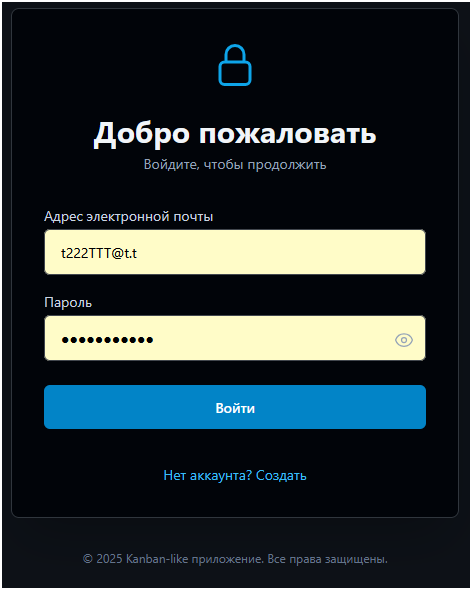
\includegraphics[width=0.7\linewidth]{окно_входа.png}}
	\caption{Окно аутентификации}
	\label{окно_входа:image}
\end{figure}

\newpage

На рисунке \ref{некорректные_данные:image} показано сообщение в случае попытки входа с неверными данными.
\begin{figure}[ht]
	\center{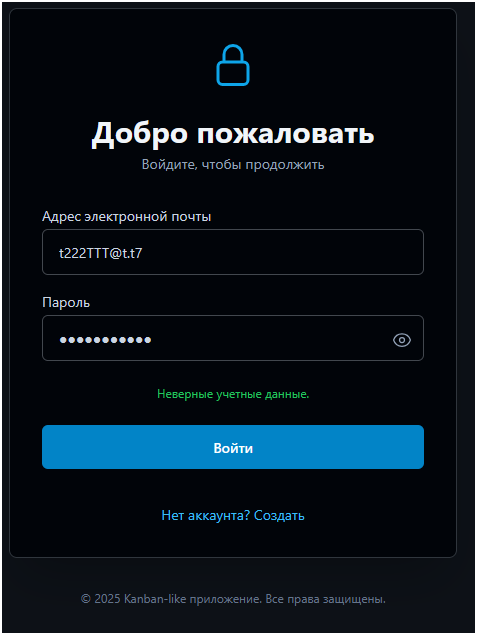
\includegraphics[width=0.7\linewidth]{некорректные_данные.png}}
	\caption{Сообщение о неверных данных}
	\label{некорректные_данные:image}
\end{figure}

\newpage

На рисунке \ref{регистрация_окно:image} показана страница с элементами для регистрации.
\begin{figure}[ht]
	\center{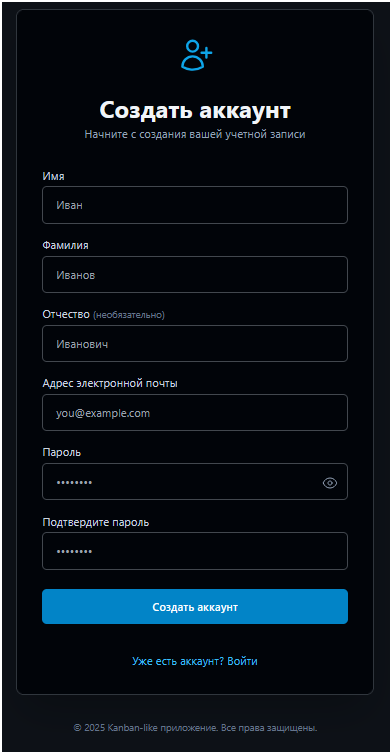
\includegraphics[width=0.6\linewidth]{регистрация_окно.png}}
	\caption{Окно регистрации}
	\label{регистрация_окно:image}
\end{figure}

\newpage

На рисунке \ref{регистрация_некорректно:image} показано сообщение в случае отсутствия заполненных полей для регистрации.
\begin{figure}[ht]
	\center{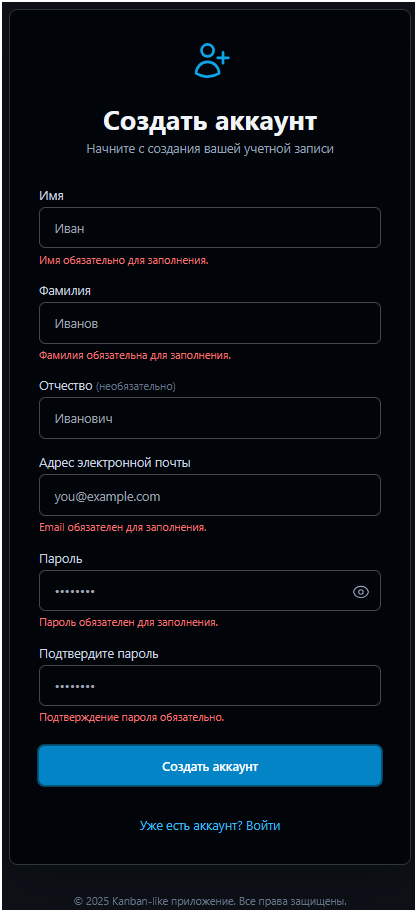
\includegraphics[width=0.6\linewidth]{регистрация_некорректно.png}}
	\caption{Проваленная валидация на заполненность полей}
	\label{регистрация_некорректно:image}
\end{figure}

\newpage

На рисунке \ref{пароль_корректно:image} показано сообщение успешной валидации пароля.
\begin{figure}[ht]
	\center{
\includegraphics[width=0.6\linewidth]{пароль_корректно.png}}
	\caption{Успешная валидация на значение пароля}
	\label{пароль_корректно:image}
\end{figure}

\newpage

На рисунке \ref{пароль_некорректно:image} показано сообщение проваленной валидации пароля.
\begin{figure}[ht]
	\center{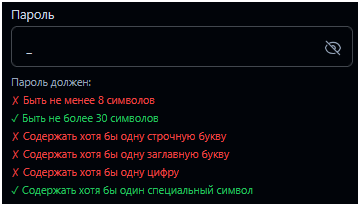
\includegraphics[width=0.6\linewidth]{пароль_некорректно.png}}
	\caption{Проваленная валидация на значение пароля}
	\label{пароль_некорректно:image}
\end{figure}

На рисунке \ref{регистрация_успешна:image} показано сообщение в случае успешной регистрации.
\begin{figure}[ht]
	\center{
\includegraphics[width=0.6\linewidth]{регистрация_успешна.png}}
	\caption{Успешная регистрациию}
	\label{регистрация_успешна:image}
\end{figure}

На рисунке \ref{окно_выхода:image} показано окно подтверждения выхода из профиля.

\newpage

\begin{figure}[ht]
	\center{
\includegraphics[width=0.6\linewidth]{окно_выхода.png}}
	\caption{Выход из профиля}
	\label{окно_выхода:image}
\end{figure}

На рисунке \ref{главная_страница:image} показана главная сраница веб-приложение.
\begin{figure}[ht]
	\center{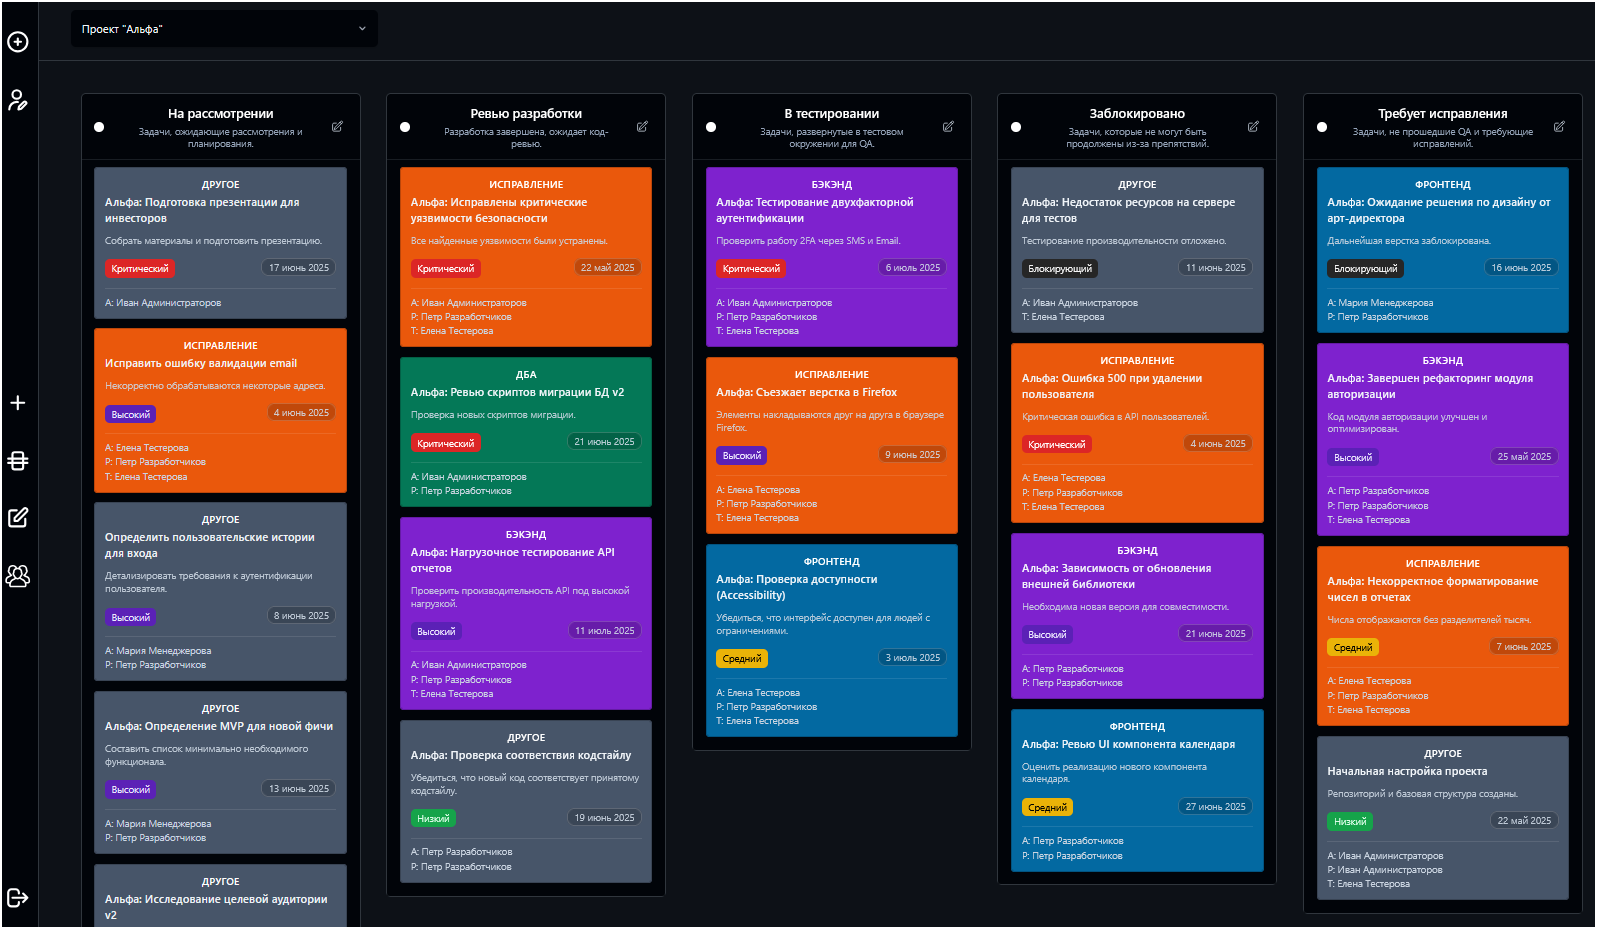
\includegraphics[width=1\linewidth]{главная_страница.png}}
	\caption{Главная страница веб-приложения}
	\label{главная_страница:image}
\end{figure}

На рисунке \ref{проект_создание:image} показано окно создания проекта.

\newpage

\begin{figure}[ht]
	\center{
\includegraphics[width=0.7\linewidth]{проект_создание.png}}
	\caption{Создание проекта}
	\label{проект_создание:image}
\end{figure}


На рисунке \ref{список_проектов:image} показано раскрываемое поле, отображающее все проекты, доступные пользователю.
\begin{figure}[ht]
	\center{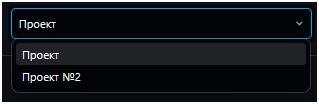
\includegraphics[width=0.7\linewidth]{список_проектов.png}}
	\caption{Список проектов}
	\label{список_проектов:image}
\end{figure}

\newpage

На рисунке \ref{проверка_надписи:image} показана поясняющая надпись у элементов панели инструментов.
\begin{figure}[ht]
	\center{
\includegraphics[width=0.5\linewidth]{проверка_надписи.png}}
	\caption{Поясняющая надпись}
	\label{проверка_надписи:image}
\end{figure}

На рисунке \ref{проект_создание_некорректно:image} показана проваленная валидация в окне создания создания проекта.
\begin{figure}[ht]
	\center{
\includegraphics[width=0.6\linewidth]{проект_создание_некорректно.png}}
	\caption{Проваленная валидация на название проекта}
	\label{проект_создание_некорректно:image}
\end{figure}

На рисунке \ref{доска_создание:image} показано окно создания доски в выбранном проекте.
\begin{figure}[ht]
	\center{
\includegraphics[width=0.6\linewidth]{доска_создание.png}}
	\caption{Создание доски}
	\label{доска_создание:image}
\end{figure}

На рисунке \ref{доска_создание_некорректно:image} показана проваленная валидация в окне создания доски.
\begin{figure}[ht]
	\center{
\includegraphics[width=0.6\linewidth]{доска_создание_некорректно.png}}
	\caption{Проваленная валидация на заголовок доски}
	\label{доска_создание_некорректно:image}
\end{figure}

На рисунке \ref{доска_создание_успешно:image} показана успешно созданная в выбранном проекте доска.
\begin{figure}[ht]
	\center{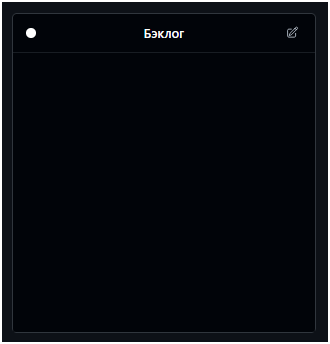
\includegraphics[width=0.6\linewidth]{доска_создание_успешно.png}}
	\caption{Успешно созданная доска}
	\label{доска_создание_успешно:image}
\end{figure}


На рисунке \ref{доска_изменение:image} показано окно редактирования доски проекта.

\newpage

\begin{figure}[ht]
	\center{
\includegraphics[width=0.6\linewidth]{доска_изменение.png}}
	\caption{Редактирование доски}
	\label{доска_изменение:image}
\end{figure}

На рисунке \ref{задача_создание:image} показано окно создания задачи в выбранном проекте.

\begin{figure}[ht]
	\center{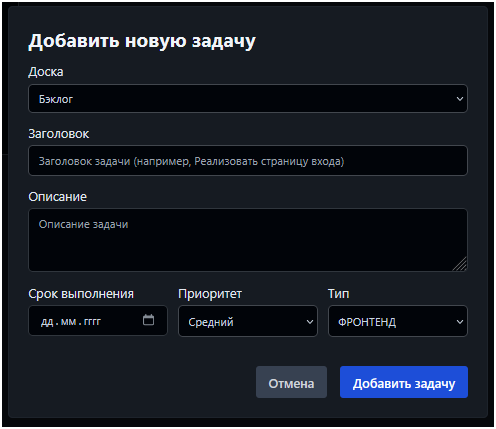
\includegraphics[width=0.6\linewidth]{задача_создание.png}}
	\caption{Создание задачи}
	\label{задача_создание:image}
\end{figure}

На рисунке \ref{задача_некорректно_заголовок:image} показана проваленная валидация на заголовок в окне создания задачи.

\newpage

\begin{figure}[ht]
	\center{
\includegraphics[width=0.6\linewidth]{задача_некорректно_заголовок.png}}
	\caption{Проваленная валидация при создании задачи}
	\label{задача_некорректно_заголовок:image}
\end{figure}

На рисунке \ref{задача_некорректно_дата:image} показана праоваленная валидация на дату сдачи в окне создания задачи.

\begin{figure}[ht]
	\center{
\includegraphics[width=0.6\linewidth]{задача_некорректно_дата.png}}
	\caption{Проваленная валидация при создании задачи}
	\label{задача_некорректно_дата:image}
\end{figure}

На рисунке \ref{задача_некорректно_доска:image} показана праоваленная валидация на доску в окне создания задачи.

\begin{figure}[ht]
	\center{
\includegraphics[width=0.6\linewidth]{задача_некорректно_доска.png}}
	\caption{Проваленная валидация при создании задачи}
	\label{задача_некорректно_доска:image}
\end{figure}

На рисунке \ref{задача_успешно:image} показано отображение успешно созданной задачи.

\begin{figure}[ht]
	\center{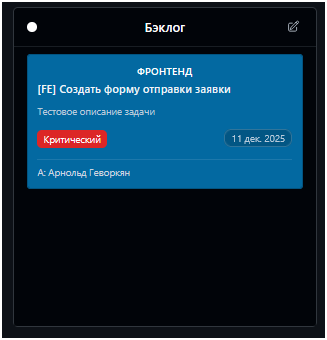
\includegraphics[width=0.6\linewidth]{задача_успешно.png}}
	\caption{Созданная задача}
	\label{задача_успешно:image}
\end{figure}

На рисунке \ref{проект_подтверждение_удаления:image} показано окно подтверждения удаления проекта.

\begin{figure}[ht]
	\center{
\includegraphics[width=0.6\linewidth]{проект_подтверждение_удаления.png}}
	\caption{Удаление проекта}
	\label{проект_подтверждение_удаления:image}
\end{figure}

На рисунках \ref{перетаскивание_задачи_1:image} и \ref{перетаскивание_задачи_2:image} показано успешное перемещение задачи между досками.

\newpage

\begin{figure}[ht]
	\center{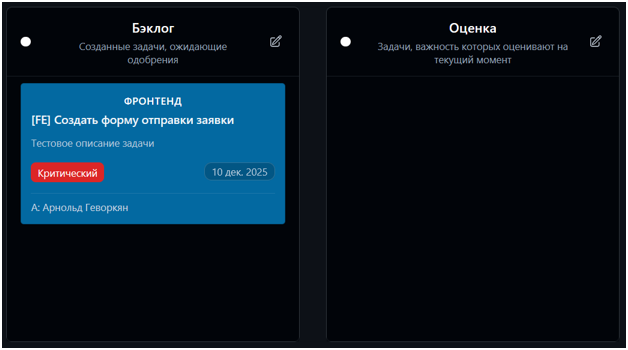
\includegraphics[width=0.6\linewidth]{перетаскивание_задачи_1.png}}
	\caption{Начальная позиция задачи}
	\label{перетаскивание_задачи_1:image}
\end{figure}

\begin{figure}[ht]
	\center{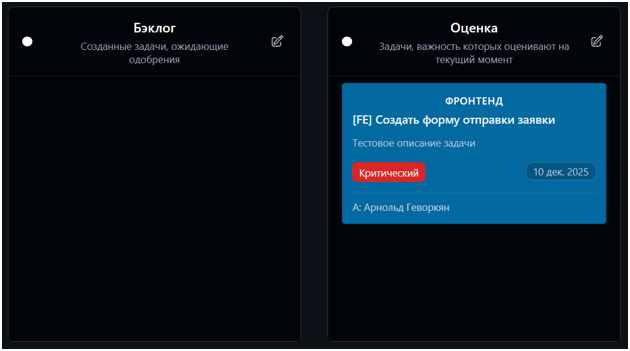
\includegraphics[width=0.6\linewidth]{перетаскивание_задачи_2.png}}
	\caption{Конечная позиция задачи}
	\label{перетаскивание_задачи_2:image}
\end{figure}

На рисунках \ref{перетаскивание_доски_1:image} и \ref{перетаскивание_доски_2:image} показано успешное перемещение досок.

\newpage

\begin{figure}[ht]
	\center{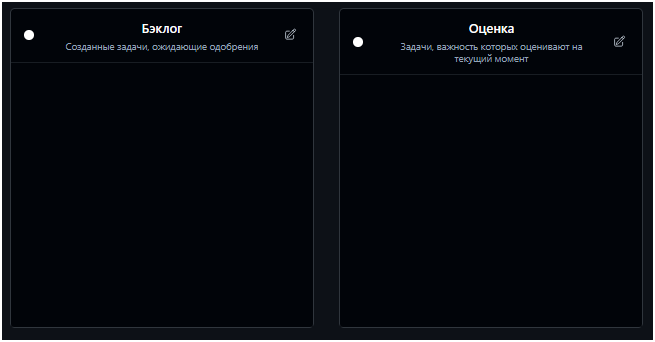
\includegraphics[width=0.6\linewidth]{перетаскивание_доски_1.png}}
	\caption{Начальные позиции досок}
	\label{перетаскивание_доски_1:image}
\end{figure}

\begin{figure}[ht]
	\center{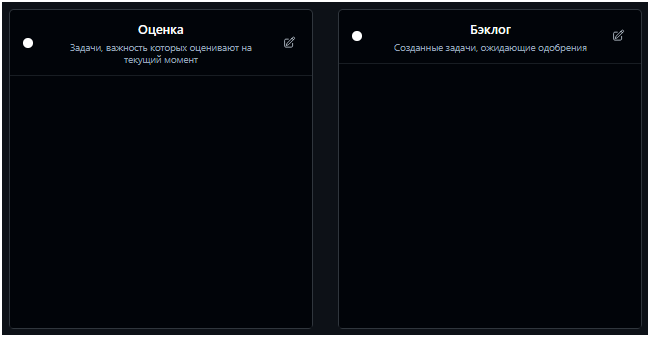
\includegraphics[width=0.6\linewidth]{перетаскивание_доски_2.png}}
	\caption{Конечные позиции досок}
	\label{перетаскивание_доски_2:image}
\end{figure}

На рисунке \ref{проект_изменение:image} показано окно редактирования проекта.
\begin{figure}[ht]
	\center{
\includegraphics[width=0.6\linewidth]{проект_изменение.png}}
	\caption{Редактирование проекта}
	\label{проект_изменение:image}
\end{figure}

На рисунке \ref{задача_просмотр:image} показано окно просмотра задачи.

\newpage

\begin{figure}[ht]
	\center{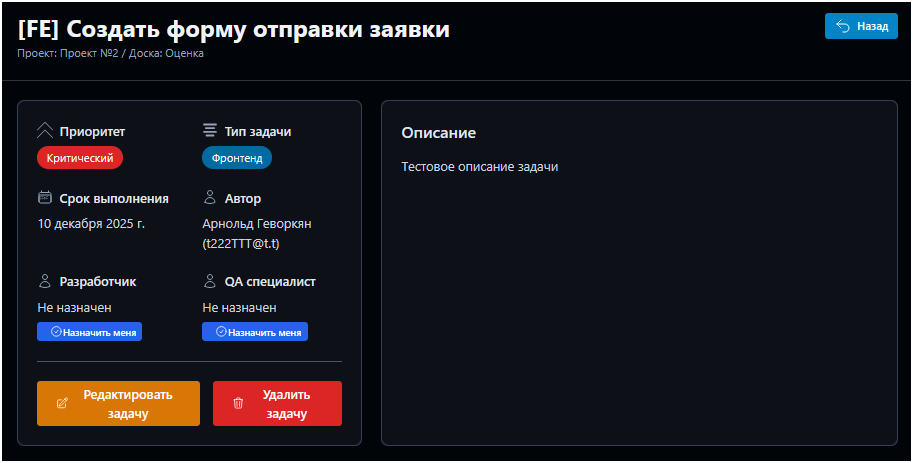
\includegraphics[width=0.9\linewidth]{задача_просмотр.png}}
	\caption{Просмотр задачи}
	\label{задача_просмотр:image}
\end{figure}

На рисунке \ref{назначение_на_роль:image} показан результат назначения пользовалтеля нароль исполнителя задачи и соответствующее сообщение.
\begin{figure}[ht]
	\center{
\includegraphics[width=0.9\linewidth]{назначение_на_роль.png}}
	\caption{Назначение на роль}
	\label{назначение_на_роль:image}
\end{figure}

На рисунке \ref{задача_изменение:image} показано окно редактирования задачи со всеми доступными полями.

\newpage

\begin{figure}[ht]
	\center{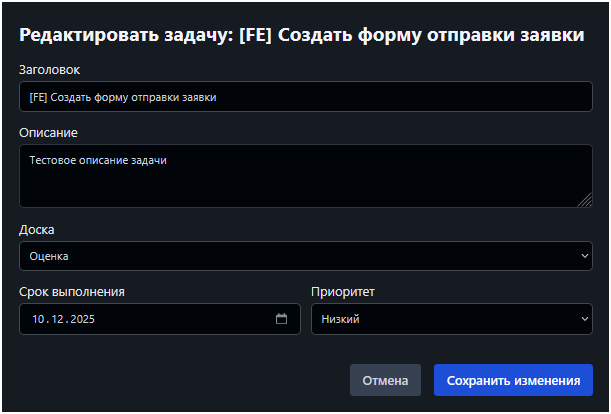
\includegraphics[width=0.6\linewidth]{задача_изменение.png}}
	\caption{Редактирование задачи}
	\label{задача_изменение:image}
\end{figure}

На рисунке \ref{задача_удаление:image} показано окно подтверждения удаления задачи.
\begin{figure}[ht]
	\center{
\includegraphics[width=0.6\linewidth]{задача_удаление.png}}
	\caption{Удаление задачи}
	\label{задача_удаление:image}
\end{figure}

На рисунке \ref{управление_окно:image} показано окно управления участниками проекта.

\newpage

\begin{figure}[ht]
	\center{
\includegraphics[width=0.6\linewidth]{управление_окно.png}}
	\caption{Участники проекта}
	\label{управление_окно:image}
\end{figure}

На рисунке \ref{управление_удаление:image} показано успешное удаление участника проекта.
\begin{figure}[ht]
	\center{
\includegraphics[width=0.6\linewidth]{управление_удаление.png}}
	\caption{Удаление участника}
	\label{управление_удаление:image}
\end{figure}

На рисунке \ref{управление_некорректно:image} показана попытка добавления несуществующего участника.

\newpage

\begin{figure}[ht]
	\center{
\includegraphics[width=0.6\linewidth]{управление_некорректно.png}}
	\caption{Ошибка добавления участника}
	\label{управление_некорректно:image}
\end{figure}

На рисунке \ref{управление_успешно:image} показано успешное добавление участника проекта.
\begin{figure}[ht]
	\center{
\includegraphics[width=0.6\linewidth]{управление_успешно.png}}
	\caption{Успешное добавление участника}
	\label{управление_успешно:image}
\end{figure}

На рисунке \ref{профиль_окно:image} показано окно профиля пользователя со всей информацией о нём.
\begin{figure}[ht]
	\center{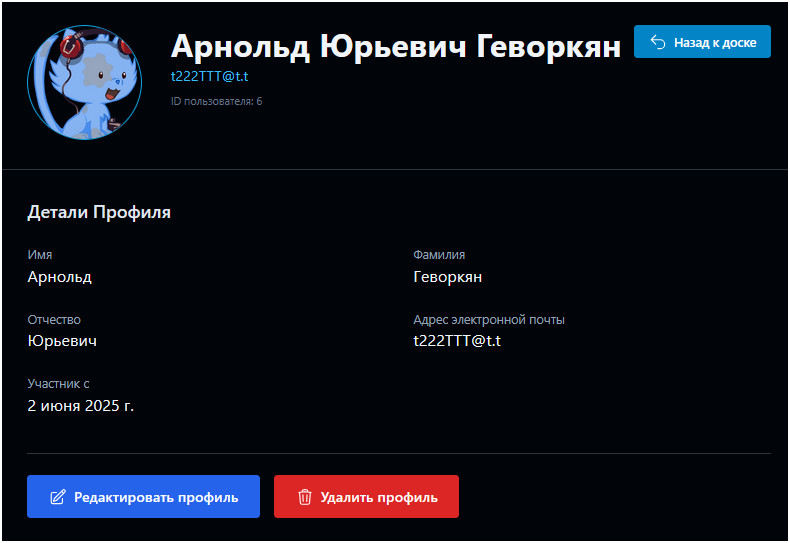
\includegraphics[width=0.6\linewidth]{профиль_окно.png}}
	\caption{Профиль пользователя}
	\label{профиль_окно:image}
\end{figure}

На рисунке \ref{профиль_редактирование:image} показано окно редактирования профиля пользователя со всеми доступными полями.

\newpage

\begin{figure}[ht]
	\center{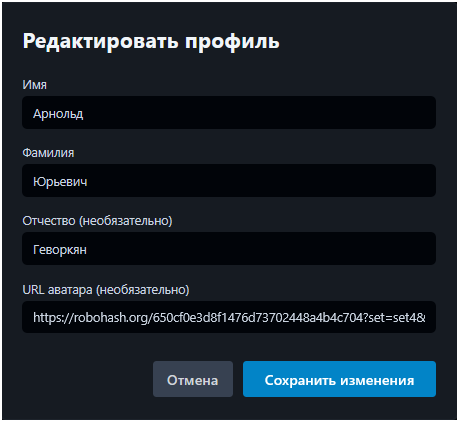
\includegraphics[width=0.6\linewidth]{профиль_редактирование.png}}
	\caption{Редактирование пользователя}
	\label{профиль_редактирование:image}
\end{figure}

На рисунке \ref{профиль_удаление:image} показано окно подтверждения удаления профиля пользователя.
\begin{figure}[ht]
	\center{
\includegraphics[width=0.6\linewidth]{профиль_удаление.png}}
	\caption{Удаление профиля}
	\label{профиль_удаление:image}
\end{figure}

На рисунке \ref{профиль_удаление_успех:image} показано оповещение об успешном удалении пользователя.
\begin{figure}[ht]
	\center{
\includegraphics[width=0.6\linewidth]{профиль_удаление_успех.png}}
	\caption{Сообщение об успешном удалении}
	\label{профиль_удаление_успех:image}
\end{figure}

\newpage

На рисунке \ref{ошибка_сессия:image} показано отображение успешно созданной задачи.
\begin{figure}[ht]
	\center{
\includegraphics[width=0.6\linewidth]{ошибка_сессия.png}}
	\caption{Ошибка валидации сессии}
	\label{ошибка_сессия:image}
\end{figure}

На рисунке \ref{конец_сессии:image} показано оповещение об истекшей сессии авторизации.

\begin{figure}[ht]
	\center{
\includegraphics[width=0.5\linewidth]{конец_сессии.png}}
	\caption{Конец сессии}
	\label{конец_сессии:image}
\end{figure}

На рисунке \ref{сортировка_проверка:image} показана сортировка задач в рамках одной доски по приоритету.

\newpage

\begin{figure}[ht]
	\center{
\includegraphics[width=0.5\linewidth]{сортировка_проверка.png}}
	\caption{Сортировка по приоритету}
	\label{сортировка_проверка:image}
\end{figure}

\newpage
\newpage